\documentclass{article}
\usepackage{graphicx}
\usepackage{booktabs}
\usepackage{float}
\usepackage{pgfplots}
\pgfplotsset{compat=1.16}
\usepackage{booktabs}

\title{Parallel Seam Carving}
\author{Luka Pantar, Mark Loboda}
\date{March 2025}

\begin{document}

\maketitle

\section{Introduction}
This report tackles the problem of parallelizing and optimizing the Seam Carving algorithm. Seam Carving is an algorithm for content-aware image resizing.

\section{Sequential algorithm}
We started development with a sequential implementation of the algorithm. The program is written to run one one \textit{CPU} core sequentially. We use this algorithm as a baseline for all the parallel implementations and for calculating the speedups of optimizations.

First, we made an optimization for the sequential algorithm. We noticed that the energy recalculation before removing a seam doesn't have to update for the whole image. We implemented an optimization where we only calculate the full image energy at the start of processing (first seam). Then after that we reuse the old calculated energies and just update the energies around the removed seam. We also had to be careful to move pixels after the removed seam one pixel to the left.

The tables \ref{tab:seq_performance} and \ref{tab:seq_performance_optimized} show a significant improvement in the total time needed to execute the program. We use the optimized algorithm as a base for all other optimizations in this report.

\begin{table}[H]
    \centering
    \scriptsize
    \begin{tabular}{lcccccc}
        \toprule
        Image & CPUs & Total Time [s] & Energy Calc. [s] & Seam Ident. [s] & Seam Annot. [s] & Seam Rem. [s] \\
        \midrule
        720x480 & 1 & 2.361027 & 2.151014 & 0.113512 & 0.000821 & 0.095657 \\
        1024x768 & 1 & 5.121556 & 4.662045 & 0.250270 & 0.001673 & 0.207538 \\
        1920x1200 & 1 & 14.998931 & 13.629237 & 0.753816 & 0.005530 & 0.610292 \\
        3840x2160 & 1 & 54.699064 & 49.597109 & 2.711426 & 0.021880 & 2.368519 \\
        7680x4320 & 1 & 223.215711 & 200.320269 & 12.368404 & 0.058917 & 10.468016 \\
        \bottomrule
    \end{tabular}
    \caption{Performance metrics for the \textit{basic sequential seam carving algorithm} without any optimizations}
    \label{tab:seq_performance}
\end{table}

\begin{table}[H]
    \centering
    \scriptsize
    \begin{tabular}{lcccccc}
        \toprule
        Image & CPUs & Total Time [s] & Energy Calc. [s] & Seam Ident. [s] & Seam Annot. [s] & Seam Rem. [s] \\
        \midrule
        720x480 & 1 & 0.566724 & 0.252795 & 0.170123 & 0.001220 & 0.142554 \\
        1024x768 & 1 & 1.033936 & 0.455606 & 0.313843 & 0.002137 & 0.262323 \\
        1920x1200 & 1 & 2.441875 & 1.048107 & 0.766809 & 0.004557 & 0.622361 \\
        3840x2160 & 1 & 8.571746 & 3.629719 & 2.707147 & 0.0212 & 2.371212\\
        7680x4320 & 1 & 38.937947 & 16.227502 & 12.314239 & 0.059571 & 10.336476 \\
        \bottomrule
    \end{tabular}
    \caption{Performance metrics for the \textit{optimized sequential seam carving algorithm}}
    \label{tab:seq_performance_optimized}
\end{table}

As we can see, the times increase drastically with higher resolutions. We want to improve that with parallelization of the algorithm.

\section{Parallel algorithms}
Parallelization was implemented using the OpenMP library in C programming language. It allows for simple parallelization of a sequential program by adding \texttt{\#pragmas} to parts of code we want to parallelize.

\subsection{Basic parallel algorithm}
This implementation takes the sequential program and adds \texttt{omp pragmas} on loops, where it is possible to parallelize the execution.

This alone improved the execution time by approximately 36\% for the largest image in our test images even with just two cores instead of one. We can also see the total execution time on one \textit{CPU} for larger images increase due to parallelization overhead.

\begin{table}[H]
    \centering
    \scriptsize
    \begin{tabular}{lccccccc}
        \toprule
        Image & CPUs & Total Time [s] & Energy Calc. [s] & Seam Ident. [s] & Seam Annot. [s] & Seam Rem. [s] \\
        \midrule
        720x480   & 1  & 0.544551  & 0.177705 & 0.220573 & 0.000901 & 0.145347 \\
        720x480   & 2  & 0.530020  & 0.151457 & 0.251664 & 0.001467 & 0.125393 \\
        720x480   & 4  & 0.331778  & 0.071489 & 0.200841 & 0.001442 & 0.057968 \\
        720x480   & 8  & 0.518315  & 0.039780 & 0.443238 & 0.002292 & 0.032945 \\
        720x480   & 16 & 0.708523  & 0.024745 & 0.661297 & 0.004160 & 0.018268 \\
        720x480   & 32 & 1.279824  & 0.033683 & 1.227879 & 0.005594 & 0.012614 \\
        \midrule
        1024x768 & 1  & 1.052977 & 0.345103 & 0.416705 & 0.001856 & 0.289282 \\
        1024x768 & 2  & 0.850637 & 0.256667 & 0.379458 & 0.002567 & 0.211914 \\
        1024x768 & 4  & 0.695689 & 0.174989 & 0.371241 & 0.003396 & 0.146018 \\
        1024x768 & 8  & 0.862765 & 0.090766 & 0.691410 & 0.005236 & 0.075287 \\
        1024x768 & 16 & 1.263389 & 0.055001 & 1.157819 & 0.008157 & 0.042356 \\
        1024x768 & 32 & 2.066088 & 0.058892 & 1.969965 & 0.012439 & 0.024743 \\
        \midrule
        1920x1200 & 1  & 3.142484 & 1.028780 & 1.224389 & 0.004678 & 0.884574 \\
        1920x1200 & 2  & 1.885429 & 0.588506 & 0.793705 & 0.004544 & 0.498593 \\
        1920x1200 & 4  & 1.253978 & 0.361863 & 0.581548 & 0.003861 & 0.306649 \\
        1920x1200 & 8  & 1.222748 & 0.188366 & 0.865899 & 0.005240 & 0.163194 \\
        1920x1200 & 16 & 1.727681 & 0.122161 & 1.508518 & 0.009520 & 0.087430 \\
        1920x1200 & 32 & 3.647868 & 0.135284 & 3.434976 & 0.015339 & 0.062225 \\
        \midrule
        3840x2160 & 1  & 11.081314 & 3.640308 & 4.238305 & 0.023160 & 3.179416 \\
        3840x2160 & 2  & 5.946992  & 1.935732 & 2.350383 & 0.019910 & 1.640867 \\
        3840x2160 & 4  & 3.382764  & 1.032482 & 1.455015 & 0.016843 & 0.878332 \\
        3840x2160 & 8  & 2.810102  & 0.563282 & 1.760398 & 0.017321 & 0.469020 \\
        3840x2160 & 16 & 3.181578  & 0.409352 & 2.460352 & 0.016426 & 0.295397 \\
        3840x2160 & 32 & 6.080257  & 0.404362 & 5.423752 & 0.032612 & 0.219488 \\
        \midrule
        7680x4320 & 1  & 46.761388 & 15.168572 & 18.108263 & 0.063444 & 13.420990 \\
        7680x4320 & 2  & 25.423843 & 8.144470  & 10.325401 & 0.063781 & 6.890088 \\
        7680x4320 & 4  & 15.607411 & 4.459218  & 7.417361  & 0.046649 & 3.684102 \\
        7680x4320 & 8  & 14.438035 & 2.930673  & 9.295500  & 0.048046 & 2.163726 \\
        7680x4320 & 16 & 14.605476 & 2.427760  & 10.468348 & 0.047523 & 1.661763 \\
        7680x4320 & 32 & 17.611841 & 1.458172  & 15.070774 & 0.060653 & 1.022156 \\
        \bottomrule
    \end{tabular}
    \caption{Performance metrics for the \textit{basic parallel seam carving algorithm}}
    \label{tab:performance_data}
\end{table}

\subsubsection{Energy calculation}
This part is straight forward to parallelize as the energy calculation of each pixel is independent and can be run in parallel. We used \texttt{\#pragma omp parallel for} which uses the default settings on the outer loop, looping through the pixel vertically. This approach was the best as each thread gets a couple of rows to calculate (as cache lines). We tried parallelizing both for loops but the results were worse.

\subsubsection{Seam identification}
This part traverses the image and calculates the minimal cumulative energy of each pixel on the path from the bottom of the image to the current pixel.

This part requires the parallelization to sync between calculation of each row in the image. The results of row \textbf{n} require the calculated result of row \textbf{n-1}. Due to parallelization of calculation of individual pixels instead of whole rows (like in other algorithm steps), the overhead grows larger than the benefits. This can be observed with all images while using more 8 or more threads.

\subsubsection{Seam removal}
This part removed the pixels on the detected seam in the image. It is trivial to parallelize as the copying can be divided into threads as the operations are fully independent of each other. We use the default \texttt{\#pragma omp parallel for}.

\subsection{Parallel seam identification}
This optimization improves the required time to execute the \textit{Seam identification} part of the algorithm by improving the parallel execution. It does that by separating pixels into triangles, where each triangle can be computed parallel as the pixels are independent in different triangles. Based on the results, it is optimal to use basic parallel algorithm while using low thread count, while opting to use triangular method for higher thread count. Triangular method is more suited for parallelization as the execution time is lower while using more threads. The height of the horizontal strip was always set to 15 pixels.

\begin{table}[H]
    \centering
    \scriptsize
    \begin{tabular}{lcccccc}
        \toprule
        Image & CPUs & Total Time [s] & Energy Calc. [s] & Seam Ident. [s] & Seam Annot. [s] & Seam Rem. [s] \\
        \midrule
        720x480 & 1 & 0.522418 & 0.172941 & 0.207059 & 0.000885 & 0.141509 \\
        720x480 & 2 & 0.474341 & 0.150984 & 0.197413 & 0.001539 & 0.124366 \\
        720x480 & 4 & 0.246060 & 0.072172 & 0.113741 & 0.001692 & 0.058418 \\
        720x480 & 8 & 0.223102 & 0.038333 & 0.149644 & 0.003584 & 0.031489 \\
        720x480 & 16 & 0.220349 & 0.023415 & 0.173959 & 0.004871 & 0.018044 \\
        720x480 & 32 & 0.335065 & 0.040527 & 0.275522 & 0.006204 & 0.012747 \\
        \midrule
        1024x768 & 1 & 1.064163 & 0.344220 & 0.429153 & 0.001835 & 0.288928 \\
        1024x768 & 2 & 0.878551 & 0.283157 & 0.357915 & 0.002587 & 0.234858 \\
        1024x768 & 4 & 0.572497 & 0.172713 & 0.252863 & 0.003475 & 0.143402 \\
        1024x768 & 8 & 0.447372 & 0.088881 & 0.276627 & 0.007978 & 0.073830 \\
        1024x768 & 16 & 0.402159 & 0.051902 & 0.301246 & 0.010575 & 0.038387 \\
        1024x768 & 32 & 0.575909 & 0.072000 & 0.463997 & 0.014086 & 0.025771 \\
        \midrule
        1920x1200 & 1 & 3.405319 & 1.005193 & 1.524670 & 0.005046 & 0.870333 \\
        1920x1200 & 2 & 1.974173 & 0.582936 & 0.891906 & 0.004961 & 0.494278 \\
        1920x1200 & 4 & 1.218669 & 0.362348 & 0.545318 & 0.003771 & 0.307158 \\
        1920x1200 & 8 & 0.938050 & 0.244778 & 0.476902 & 0.007385 & 0.208939 \\
        1920x1200 & 16 & 0.731339 & 0.138578 & 0.458428 & 0.010968 & 0.123325 \\
        1920x1200 & 32 & 1.069391 & 0.134886 & 0.842450 & 0.017889 & 0.074120 \\
        \midrule
        3840x2160 & 1 & 12.977201 & 3.633735 & 6.142827 & 0.023129 & 3.177378 \\
        3840x2160 & 2 & 6.766262 & 1.931479 & 3.165322 & 0.019858 & 1.649516 \\
        3840x2160 & 4 & 3.613572 & 1.039246 & 1.680265 & 0.016987 & 0.876991 \\
        3840x2160 & 8 & 2.293358 & 0.591426 & 1.188656 & 0.019149 & 0.494044 \\
        3840x2160 & 16 & 1.744437 & 0.422771 & 0.952499 & 0.015968 & 0.353152 \\
        3840x2160 & 32 & 1.893399 & 0.338638 & 1.304256 & 0.027705 & 0.222771 \\
        \midrule
        7680x4320 & 1 & 54.551780 & 15.162716 & 25.913204 & 0.062464 & 13.413288 \\
        7680x4320 & 2 & 28.600833 & 8.150284 & 13.517435 & 0.062234 & 6.870766 \\
        7680x4320 & 4 & 18.369055 & 4.432420 & 10.232190 & 0.046913 & 3.657454 \\
        7680x4320 & 8 & 14.170526 & 2.918553 & 9.087091 & 0.048002 & 2.116800 \\
        7680x4320 & 16 & 14.115907 & 2.464454 & 9.968934 & 0.048545 & 1.633897 \\
        7680x4320 & 32 & 11.023667 & 1.441946 & 8.608425 & 0.057640 & 0.915584 \\
        \bottomrule
    \end{tabular}
    \caption{Performance metrics for \textit{parallel seam carving algorithm} with \textit{parallel seam identification}}
    \label{tab:performance}
\end{table}

\subsection{Parallel seam removal}
This optimization improves the required time to execute the \textit{Seam removal} part of the algorithm. The greedy approach was implemented by splitting the image in column strips and finding/removing a seam on each of the strips. The number of simultaneous number of removed seams in each iteration was set to 8.

\begin{table}[H]
    \centering
    \scriptsize
    \begin{tabular}{lccccccc}
        \toprule
        Image & CPUs & Total Time [s] & Energy Calc. [s] & Seam Ident. [s] & Seam Annot. [s] & Seam Rem. [s] \\
        \midrule
        720x480  & 1  & 0.155218 & 0.070204 & 0.053218 & 0.000452 & 0.031339 \\
        720x480  & 2  & 0.088558 & 0.035751 & 0.036767 & 0.000245 & 0.015789 \\
        720x480  & 4  & 0.057260 & 0.018495 & 0.030546 & 0.000155 & 0.008059 \\
        720x480  & 8  & 0.081664 & 0.010894 & 0.065302 & 0.000219 & 0.005239 \\
        720x480  & 16 & 0.117620 & 0.007895 & 0.105922 & 0.000494 & 0.003300 \\
        720x480  & 32 & 0.185901 & 0.009234 & 0.173239 & 0.000692 & 0.002728 \\
        \midrule
        1024x768 & 1  & 0.348044 & 0.156742 & 0.117819 & 0.000755 & 0.072719 \\
        1024x768 & 2  & 0.187911 & 0.079689 & 0.071465 & 0.000390 & 0.036362 \\
        1024x768 & 4  & 0.116837 & 0.041749 & 0.056415 & 0.000247 & 0.018421 \\
        1024x768 & 8  & 0.129605 & 0.023932 & 0.092722 & 0.000286 & 0.012657 \\
        1024x768 & 16 & 0.194703 & 0.016092 & 0.171351 & 0.000783 & 0.006465 \\
        1024x768 & 32 & 0.297025 & 0.018766 & 0.272316 & 0.001080 & 0.004850 \\
        \midrule
        1920x1200 & 1  & 0.818145 & 0.374116 & 0.270256 & 0.001441 & 0.172324 \\
        1920x1200 & 2  & 0.579903 & 0.249701 & 0.209017 & 0.000804 & 0.120367 \\
        1920x1200 & 4  & 0.302969 & 0.117925 & 0.129146 & 0.000504 & 0.055382 \\
        1920x1200 & 8  & 0.259953 & 0.063370 & 0.166001 & 0.000574 & 0.029996 \\
        1920x1200 & 16 & 0.307365 & 0.040673 & 0.248535 & 0.000820 & 0.017327 \\
        1920x1200 & 32 & 0.474478 & 0.040516 & 0.416702 & 0.002077 & 0.015173 \\
        \midrule
        3840x2160 & 1  & 2.120121 & 0.987060 & 0.674265 & 0.017090 & 0.441691 \\
        3840x2160 & 2  & 1.822199 & 0.788763 & 0.632257 & 0.009449 & 0.391715 \\
        3840x2160 & 4  & 1.420209 & 0.437198 & 0.765366 & 0.004271 & 0.213364 \\
        3840x2160 & 8  & 0.722427 & 0.236375 & 0.362043 & 0.004626 & 0.119371 \\
        3840x2160 & 16 & 0.618702 & 0.114680 & 0.445355 & 0.005520 & 0.053134 \\
        3840x2160 & 32 & 0.866082 & 0.097409 & 0.714602 & 0.006079 & 0.047983 \\
        \midrule
        7680x4320 & 1  & 7.967661 & 3.470477 & 2.693971 & 0.041115 & 1.762084 \\
        7680x4320 & 2  & 4.993922 & 2.297811 & 1.687800 & 0.021230 & 0.987069 \\
        7680x4320 & 4  & 3.321433 & 1.367542 & 1.307329 & 0.009190 & 0.637361 \\
        7680x4320 & 8  & 2.565144 & 0.833502 & 1.312234 & 0.008986 & 0.410411 \\
        7680x4320 & 16 & 2.224144 & 0.475441 & 1.495399 & 0.009520 & 0.243774 \\
        7680x4320 & 32 & 2.747093 & 0.358370 & 2.180716 & 0.009253 & 0.198741 \\
        \bottomrule
    \end{tabular}
    \caption{Performance metrics for the \textit{parallel seam carving algorithm} with \textit{parallel seam removal}}
    \label{tab:performance_data_new}
\end{table}


\section{Results}

\subsection{Speed ups relative to the base sequential seam removal algorithm}
% Table of Sequential, Parallel Times and Speedup
\begin{table}[H]
    \centering
    \caption{Performance Metrics for the Seam Carving Algorithm}
    \begin{tabular}{lccccc}
        \toprule
        Image Size & Optimal CPUs & Sequential Time (s) & Parallel Time (s) & Speedup \\
        \midrule
        720x480   & 16           & 2.361027            & 0.220349          & 10.72  \\
        1024x768  & 16           & 5.121556            & 0.402159          & 12.74  \\
        1920x1200 & 16           & 14.998931           & 0.731339          & 20.51  \\
        3840x2160 & 16           & 54.699064           & 1.744437          & 31.36  \\
        7680x4320 & 32           & 223.215711          & 11.023667         & 20.26  \\
        \bottomrule
    \end{tabular}
    \label{tab:performance_summary}
\end{table}

% Plot for Speedup
\begin{figure}[H]
    \centering
    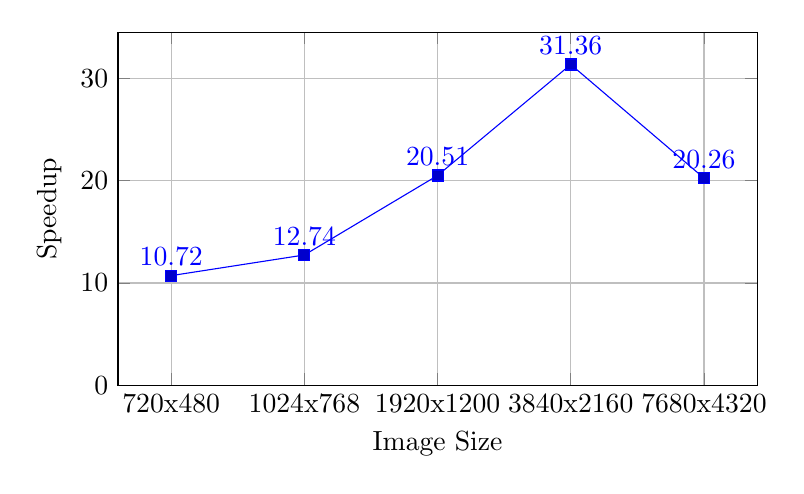
\begin{tikzpicture}
        \begin{axis}[
            width=0.8\textwidth,
            height=0.5\textwidth,
            xlabel={Image Size},
            ylabel={Speedup},
            xtick=data,
            symbolic x coords={720x480,1024x768,1920x1200,3840x2160,7680x4320},
            nodes near coords,
            ymin=0,
            grid=both,
        ]
        \addplot+[mark=square*] coordinates {
            (720x480,10.72)
            (1024x768,12.74)
            (1920x1200,20.51)
            (3840x2160,31.36)
            (7680x4320,20.26)
        };
        \end{axis}
    \end{tikzpicture}
    \caption{Speedup vs. Image Size}
    \label{fig:speedup_plot}
\end{figure}

\subsection{Speed ups relative to the optimized sequential seam removal algorithm}

\begin{table}[H]
\centering
\scriptsize
\begin{tabular}{lccccc}
    \toprule
    Image      & Optimal CPUs & Sequential Time [s] & Parallel Time [s] & Speedup \\
    \midrule
    720$\times$480    & 16 & 0.566724 & 0.220349 & 2.57 \\
    1024$\times$768   & 16 & 1.033936 & 0.402159 & 2.57 \\
    1920$\times$1200  & 16 & 2.441875 & 0.731339 & 3.34 \\
    3840$\times$2160  & 16 & 8.571746 & 1.744437 & 4.92 \\
    7680$\times$4320  & 32 & 38.937947 & 11.023667 & 3.53 \\
    \bottomrule
\end{tabular}
\caption{Speedup of Parallel Seam Carving Algorithm relative to base sequential seam removal algorithm by image size}
\label{tab:speedup-optimized}
\end{table}

\begin{figure}[H]
    \centering
    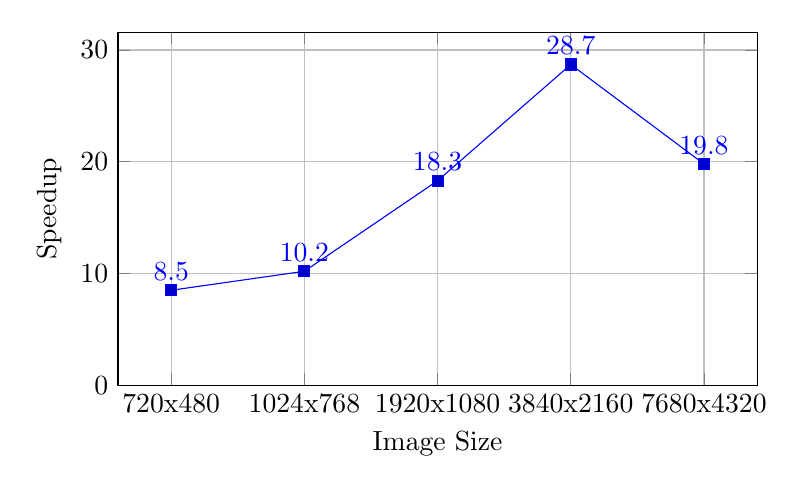
\begin{tikzpicture}
        \begin{axis}[
            width=0.8\textwidth,
            height=0.5\textwidth,
            xlabel={Image Size},
            ylabel={Speedup},
            xtick=data,
            symbolic x coords={720x480,1024x768,1920x1080,3840x2160,7680x4320},
            nodes near coords,
            ymin=0,
            grid=both,
        ]
        \addplot+[mark=square*] coordinates {
            (720x480,8.5)
            (1024x768,10.2)
            (1920x1080,18.3)
            (3840x2160,28.7)
            (7680x4320,19.8)
        };
        \end{axis}
    \end{tikzpicture}
    \caption{Speedup of Parallel Seam Carving Algorithm relative to optimized sequential seam removal algorithm by image size.}
    \label{fig:speedup_seam_carving}
\end{figure}


\end{document}


\section{Conclusion}
\subsection{Result interpretation}
\subsection{Future improvements}

\end{document}
